\subsection{Paths, centrality and spreading}\label{sec:r-function}
% Owner: D
% M3a - Temporal Reachability

\begin{figure}[t]
    \centering
    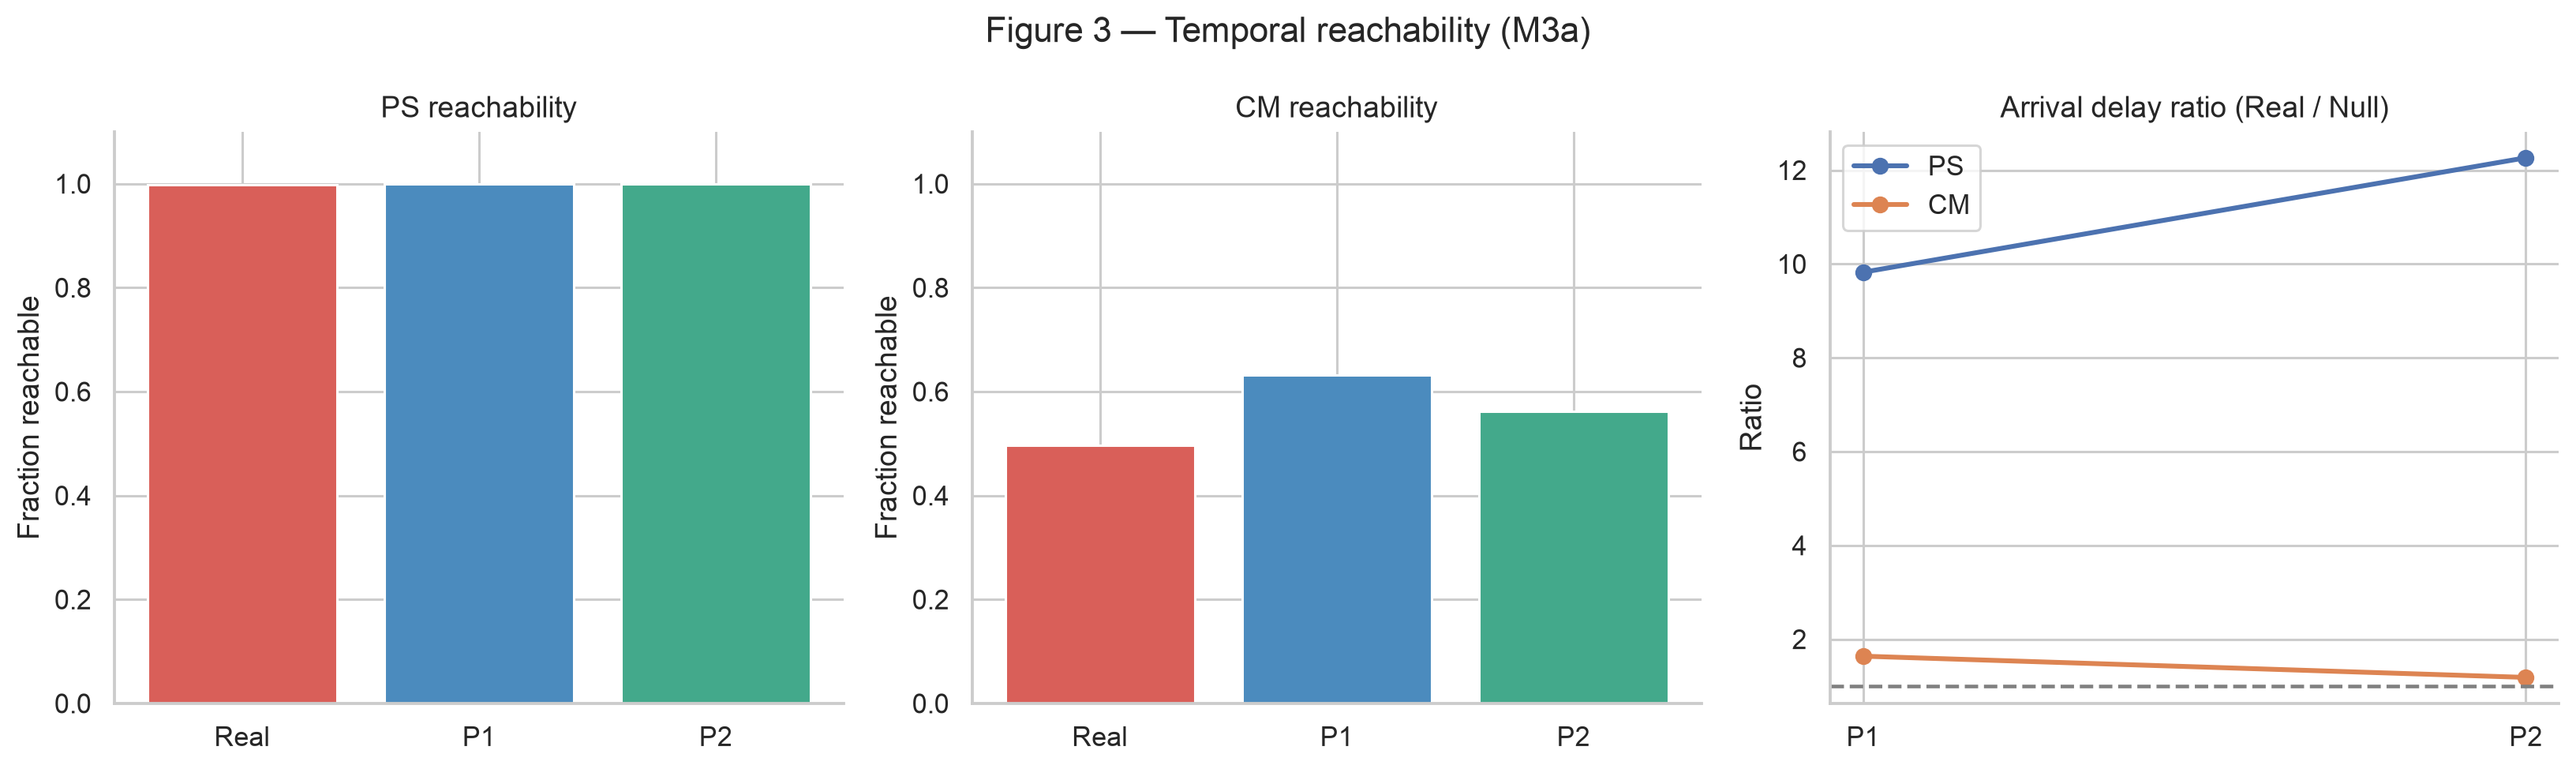
\includegraphics[width=\linewidth]
    {Fig3_reachability_and_delay.png}
    \caption{Temporal reachability comparison
    between real and randomized networks.}
    \label{fig:d_reachability}
\end{figure}

% 后面继续放你的完整M3a实验分析
% =========================================================
% Member D: M3a Temporal Reachability and M3c SIR Spreading
% =========================================================

\subsubsection{Temporal Reachability (M3a)}
\label{sec:d_reachability}

We first investigate H6a: temporal ordering restricts
network reachability. We compare the original temporal
networks (Real) with timestamp-shuffled (P1) and
edge-randomized (P2) reference networks.

Two metrics are considered: temporal reachability and
mean earliest-arrival delay. The former measures the
fraction of reachable nodes under time-respecting paths,
while the latter measures the time required to reach
accessible destinations.

\paragraph{Reachability results.}

Figure~\ref{fig:d_reachability} presents the temporal
reachability results for the Primary School (PS) and
CollegeMsg (CM) datasets.

\begin{figure*}[t]
    \centering
    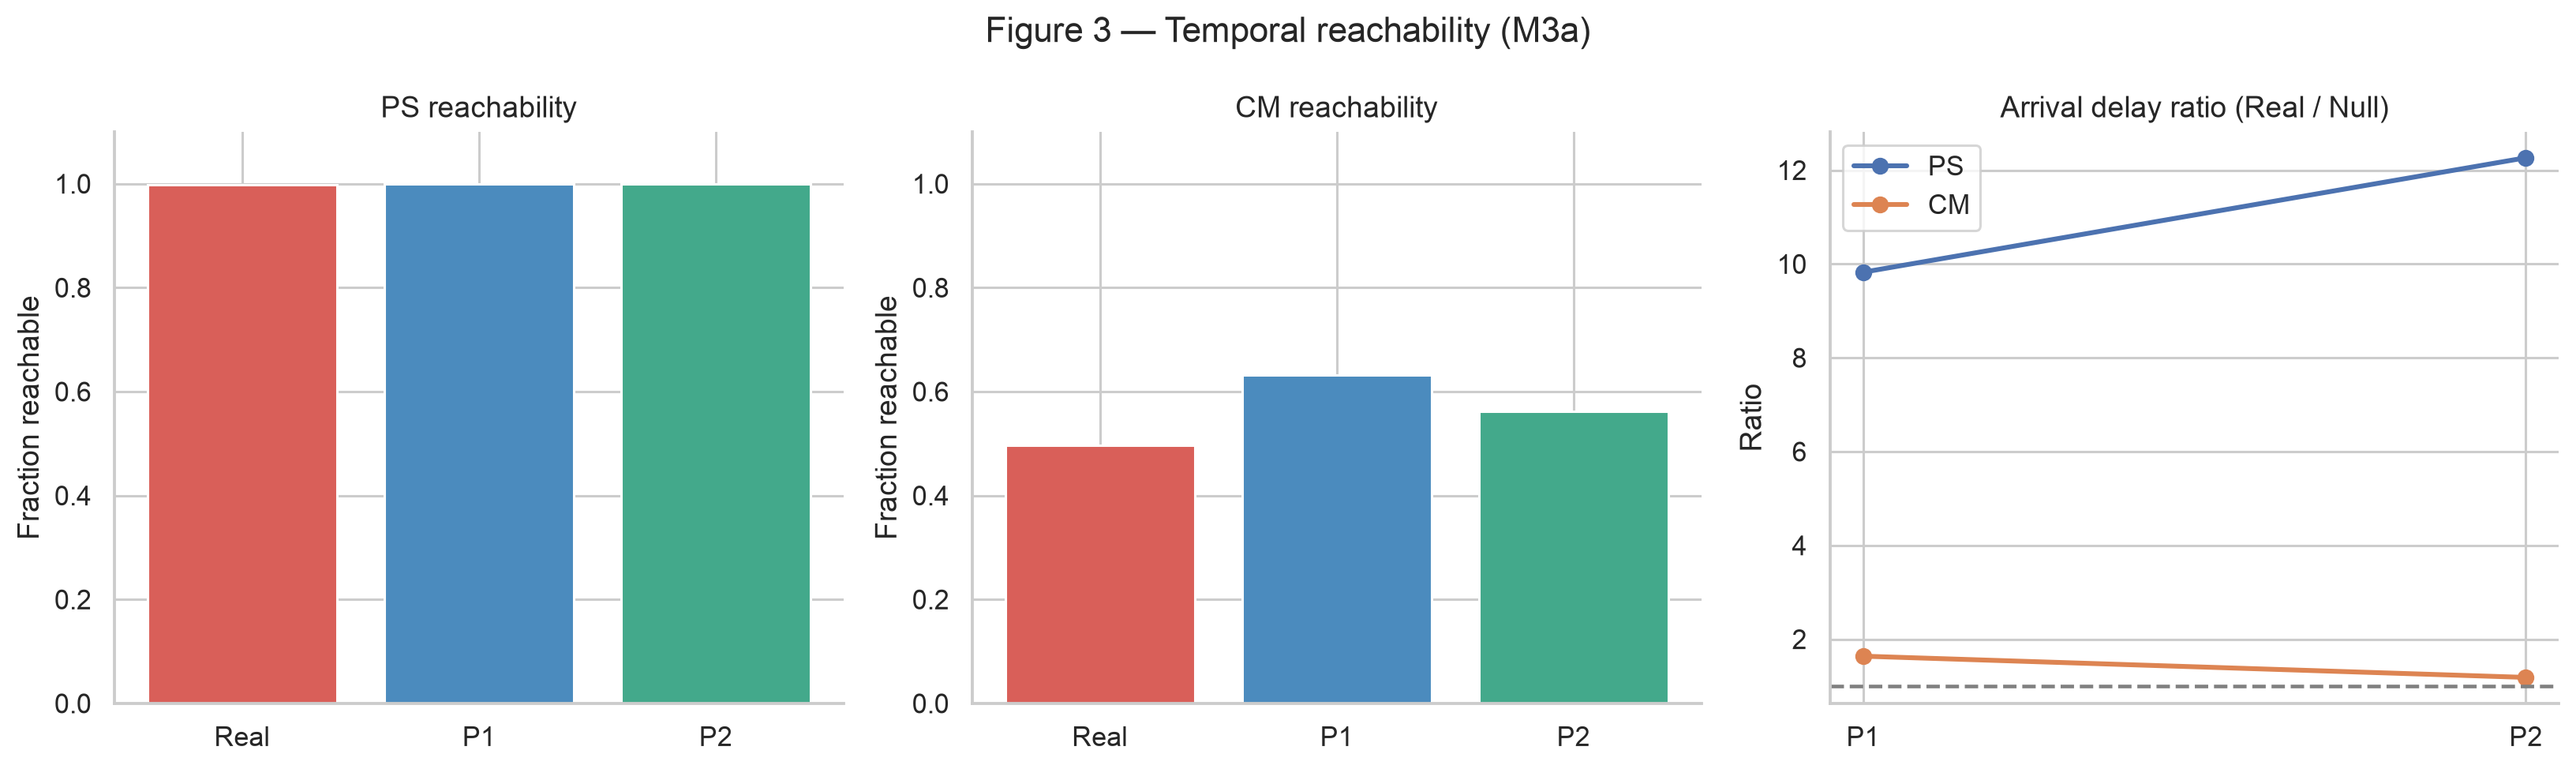
\includegraphics[width=0.85\textwidth]
    {Fig3_reachability_and_delay.png}
    \caption{Temporal reachability analysis (M3a).
    The first two panels show reachability in PS and CM.
    The third panel compares the real-to-null arrival-delay
    ratios. Ratios above one indicate longer arrival delays
    in the original temporal network.}
    \label{fig:d_reachability}
\end{figure*}

In PS, the real network achieves a reachability ratio
of 0.9981, compared with 1.0000 for both P1 and P2.
Thus, almost all nodes remain temporally reachable
regardless of randomization.

However, the mean arrival delay differs substantially.
The real-network delay is approximately 9.82 times
that of P1 and 12.26 times that of P2.

This indicates that temporal ordering does not
necessarily prevent nodes from being reached,
but can considerably delay information propagation.

In CM, the real reachability ratio is 0.4965,
compared with 0.6326 for P1 and 0.5618 for P2.

Relative to P1, reachability decreases by
approximately 21.5\%, while the reduction
relative to P2 is approximately 11.6\%.

The real-network mean arrival delay is also
1.64 times that of P1 and 1.19 times that of P2.

Unlike PS, CM therefore exhibits substantial
differences in both temporal reachability
and arrival delay.

\begin{table}[t]
\centering
\caption{Temporal reachability and normalized
arrival-delay results for M3a.}
\label{tab:d_reachability}
\small
\begin{tabular}{lccc}
\toprule
Dataset & Real & P1 & P2 \\
\midrule
PS reachability & 0.9981 & 1.0000 & 1.0000 \\
CM reachability & 0.4965 & 0.6326 & 0.5618 \\
\midrule
\multicolumn{4}{c}{Arrival-delay ratios} \\
\midrule
Dataset & Real/P1 & Real/P2 & \\
PS & 9.82 & 12.26 & \\
CM & 1.64 & 1.19 & \\
\bottomrule
\end{tabular}
\end{table}

\paragraph{Verdict on H6a.}

The results provide descriptive support for H6a
in both datasets. In PS, temporal ordering mainly
increases arrival delays, whereas in CM it reduces
reachability and increases delays.

Therefore, the influence of temporal ordering
depends on the interaction patterns and temporal
organization of the network.
% Owner: E. M3b / H6 (rankings), input from results_function.tex.
% Values: results/e_summary.csv and results/e/m3b_*; figure: scripts/plot_e.py.
\begin{table}[t]
\centering
\small
\begin{tabular}{@{}llcc@{}}
\toprule
 & Measure & Real & P1 \\
\midrule
PS & $\tau$, unweighted & 0.71 & $0.55\pm0.01$ \\
   & $\tau$, weighted & 0.39 & $0.69\pm0.01$ \\
   & top-10\%, unweighted & 0.50 & $0.51\pm0.07$ \\
   & top-10\%, weighted & 0.29 & $0.60\pm0.06$ \\
\midrule
CM & $\tau$, unweighted & 0.78 & $0.85\pm0.00$ \\
   & $\tau$, weighted & 0.74 & $0.86\pm0.00$ \\
   & top-10\%, unweighted & 0.65 & $0.74\pm0.01$ \\
   & top-10\%, weighted & 0.57 & $0.72\pm0.02$ \\
\bottomrule
\end{tabular}
\caption{Agreement of static and temporal closeness rankings: Kendall $\tau_b$ and
overlap of the top 10\% nodes. P1: temporal closeness on 20 samples (mean $\pm$ sd); the
static ranking is unchanged by P1.}
\label{tab:m3b}
\end{table}

\begin{figure*}[t]
\centering
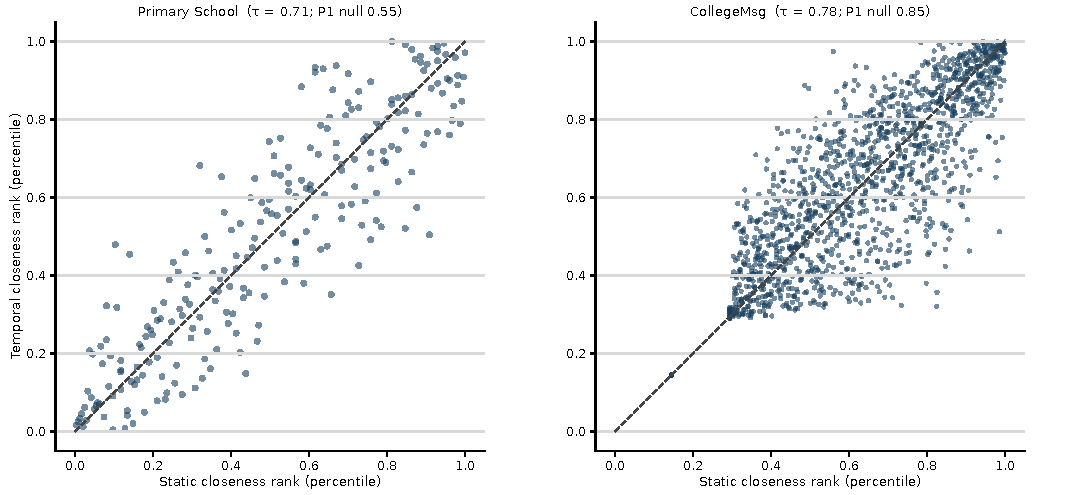
\includegraphics[width=0.8\linewidth]{e_m3b_rank_scatter.pdf}
\caption{Static (unweighted harmonic) vs.\ temporal closeness rank of every node; dashed:
identical rankings. The tied block at the lower left of the CM panel is the 29\% of users
who never send a message.}
\label{fig:m3b}
\end{figure*}

\paragraph{Centrality.}
Static and temporal closeness rankings are clearly correlated in both networks
(\cref{tab:m3b,fig:m3b}; $\tau=0.71$ in PS and $0.78$ in CM, hop distance), so the static
network shows roughly which nodes are central. It is much less reliable about which nodes
are \emph{most} central: only half of the PS top 10\% and two thirds of the CM top 10\%
coincide. In CM the real agreement is somewhat lower than under P1 (0.78 vs.\ 0.85), so
event order makes static closeness a slightly worse guide. The CM $\tau$ is also helped by
the 549 users (29\%) who never send a message and have zero closeness in both rankings
(the tied block in \cref{fig:m3b}).

In PS the effect depends on edge weights. Weighted static closeness agrees poorly with
temporal closeness ($\tau=0.39$, top-10\% overlap 0.29), whereas after P1 the agreement
is high ($0.69\pm0.01$). In the school, most contact weight comes from repeated contacts
within a class during lessons; these happen while the class is already connected and
hardly shorten time-respecting paths to the rest of the school. Under P1 the same contacts
are spread over the day, and a heavy edge becomes a frequent chance to transmit. Without
weights the effect reverses (real 0.71 vs.\ P1 0.55): reaching the school quickly depends
on having many distinct partners, which in PS largely means mixing at breaks.

\emph{Rankings part of H6: partly supported.} The rankings are correlated
($\tau=0.71$--$0.78$) but the top nodes differ by 35--50\%, and in face-to-face data
weighting edges by contact frequency makes the static ranking misleading ($\tau=0.39$).

% Owner: D. Event-started SIR; supersedes the observation-start experiment.
\paragraph{Event-driven SIR (M3c).}\label{sec:d_sir}
Each network uses 200 seeds at randomly selected events in its first 70\% of event
positions. CM seeds use the sender; PS randomly selects either endpoint. The selected
seed event itself is excluded by the strict-time convention. Infectious duration is
fixed, transmission probability is per record, and recovered nodes remain immune.
Final size includes the seed. A major outbreak reaches at least 5\% of period nodes.
Peak delays are averaged over major outbreaks only; $T_{\rm real}/\overline T_{\rm null}$
is a conditional ratio of means. Nulls with no major outbreaks give an undefined peak,
not a zero delay. Simultaneous infections and recoveries are grouped before measuring
prevalence; the earliest maximum is selected.
\begin{table*}[!htbp]\centering\small
\begin{tabular}{@{}llrrrrrrrr@{}}
\toprule & & \multicolumn{3}{c}{Final infected fraction} & \multicolumn{3}{c}{Major outbreak probability} & \multicolumn{2}{c}{Peak ratio} \\
Dataset & $(\beta,D)$ & Real & P1 & P2 & Real & P1 & P2 & vs P1 & vs P2 \\
\midrule
PS & (0.05, 4 h) & 0.629 & 0.776 & 0.823 & 0.860 & 0.908 & 0.920 & 1.160 & 1.214 \\
PS & (0.02, 4 h) & 0.373 & 0.420 & 0.559 & 0.700 & 0.754 & 0.778 & 1.000 & 1.088 \\
PS & (0.1, 4 h) & 0.734 & 0.893 & 0.918 & 0.910 & 0.960 & 0.973 & 1.311 & 1.340 \\
PS & (0.05, 1 h) & 0.373 & 0.634 & 0.674 & 0.745 & 0.844 & 0.852 & 1.021 & 1.265 \\
CM & (0.2, 336 h) & 0.256 & 0.250 & 0.276 & 0.825 & 0.791 & 0.799 & 0.888 & 0.995 \\
CM & (0.05, 336 h) & 0.026 & 0.013 & 0.025 & 0.215 & 0.082 & 0.192 & 0.934 & 0.991 \\
CM & (0.5, 336 h) & 0.460 & 0.506 & 0.530 & 0.975 & 0.954 & 0.965 & 0.924 & 0.982 \\
CM & (0.2, 72 h) & 0.074 & 0.043 & 0.066 & 0.555 & 0.342 & 0.428 & 0.720 & 1.013 \\
\bottomrule\end{tabular}
\caption{Four SIR settings per dataset, 200 seeds per network, 20 nulls per family.
The first setting in each dataset is primary. The peak-ratio population is restricted
to major outbreaks and can differ between real and null networks.}\label{tab:d-sir}
\end{table*}
\begin{figure*}[!htbp]
\centering
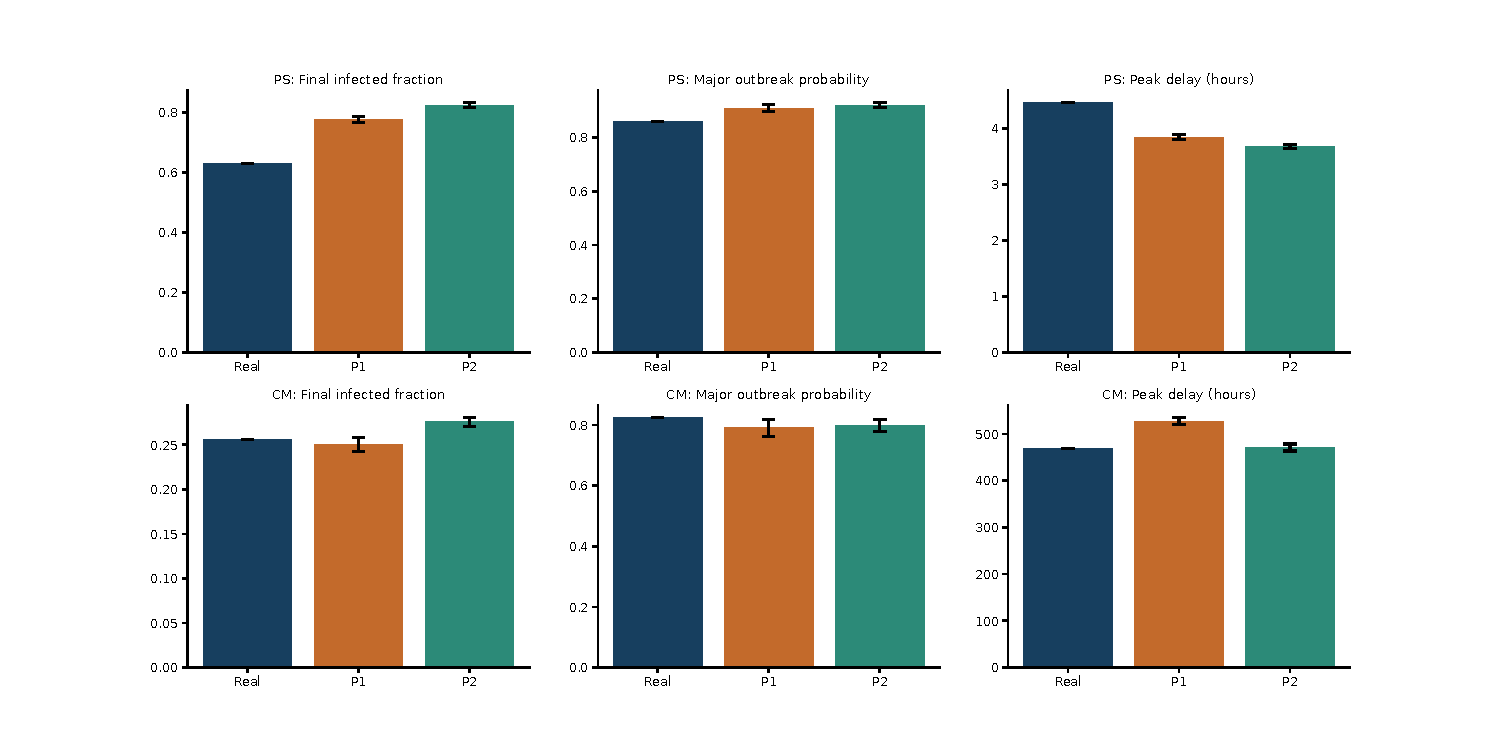
\includegraphics[width=\linewidth]{d_sir_event_seeds.pdf}
\caption{Primary SIR settings. Peak delay is conditional on major outbreaks; errors describe null-network variation.}
\label{fig:d_sir}
\end{figure*}
The revised design produces nontrivial CM outbreaks. Absence of secondary infections
in the earlier run arose from infecting seeds at the observation boundary with an
unsuitable short duration; it is not evidence for an intrinsic property of CM.

\paragraph{Parameter, null and outcome dependence.}
For PS versus P1, the peak ratio is 1.0005 at $\beta=.02$ (negligible peak difference),
1.160 at .05 and 1.311 at .10 for a four-hour infectious duration. Final size is
lower than both null families in all four tested settings; at the primary setting
it is 0.629 versus P1 0.776. The qualifying populations also differ: major outbreaks
occur for 0.860 of real seeds versus a mean 0.908 under P1. Conditional peak comparisons
therefore use different seed subsets and are not paired-seed causal slowdowns.

CM peaks earlier than P1 across the full-period settings (ratios 0.72--0.94),
whereas P2 peak ratios are approximately 0.98--1.01. Even the choice of timing
metric matters: at $\beta=.5$, 14 days, the peak ratio to P1 is 0.924 but the
half-final-size time ratio is 1.061. The latter is time to half of each trajectory's
own final infected count, not time to a common epidemic size. These opposing signs
exclude a general claim that the entire spreading process is faster or slower.
In CM's second half, two weaker settings have no major real outbreaks (undefined
peak ratios); the primary setting still has major-outbreak probability 0.360.

PS's real mean final fraction is 0.629 over the full interval versus 0.821/0.788
in the halves. Uniform sampling from the first 70\% of each event stream changes
seed identities, start positions and residual observation horizons when the interval
is split. Finite horizons and schedule boundaries may contribute; these CSV comparisons
alone do not identify their contribution separately. These are protocol sensitivities,
not evidence that truncating the data intrinsically strengthens propagation.

\paragraph{Verdict on H6 and H7.}
H6's reachability component is supported under the multi-start protocol in both datasets;
rankings show a partial effect, with correlated rankings but different top nodes.
H7 is conditional on parameters and the reference model. PS peaks later under its
primary setting; CM peaks earlier than P1 across the four tested full-period settings and is close
to P2. The claim that slowing is strongest in CM is therefore not supported.
Peak timing among major outbreaks does not by itself measure population-wide epidemic speed.
